\section{Materiales y métodos}

%Para el circuito RC se buscó determinar la frecuencia de corte $\omega_c$, definida como aquella para la cual la función de transferencia cumple $|H(\omega_c)|= \frac{1}{\sqrt{2}}$, lo que corresponde a una disminución de la potencia a la mitad, dado que $P\propto |H|^2$. Utilizando el hecho de que en los regímenes de bajas y altas frecuencias la función $H(\omega)$ presenta comportamientos simples (aproximadamente constante en uno de los extremos y proporcional a una potencia de $\omega$ ($\omega$ para el pasa altos y $\omega^{-1}$ para el pasa bajos en el otro), que se traducen en rectas en escala logarítmica,  se representó el $\text{log}(H)$ en función del $\text{log}(\omega)$. Fueron realizados ajustes lineales en las dos regiones diferenciadas, estimando la frecuencia de corte a partir de la intersección de dichas rectas, pues es una buena aproximación al punto donde la función $|H(\omega)|$ alcanza el valor $\frac{1}{\sqrt{2}}$.  

 Se estudiaron dos circuitos en serie: un circuito RC y un circuito RLC. Para ambos se utilizó una resistencia de \SI{1,00(5)}{\kilo\ohm}, y un capacitor de \SI{100(10)}{\nano\farad} comerciales y, para el caso del circuito RLC, un inductor $L$ de inductancia desconocida (ver \autoref{fig:ambosCircuitos}).
 
 \begin{figure}[H]
    \centering
    \begin{subfigure}[b]{0.45\linewidth}
        \centering
        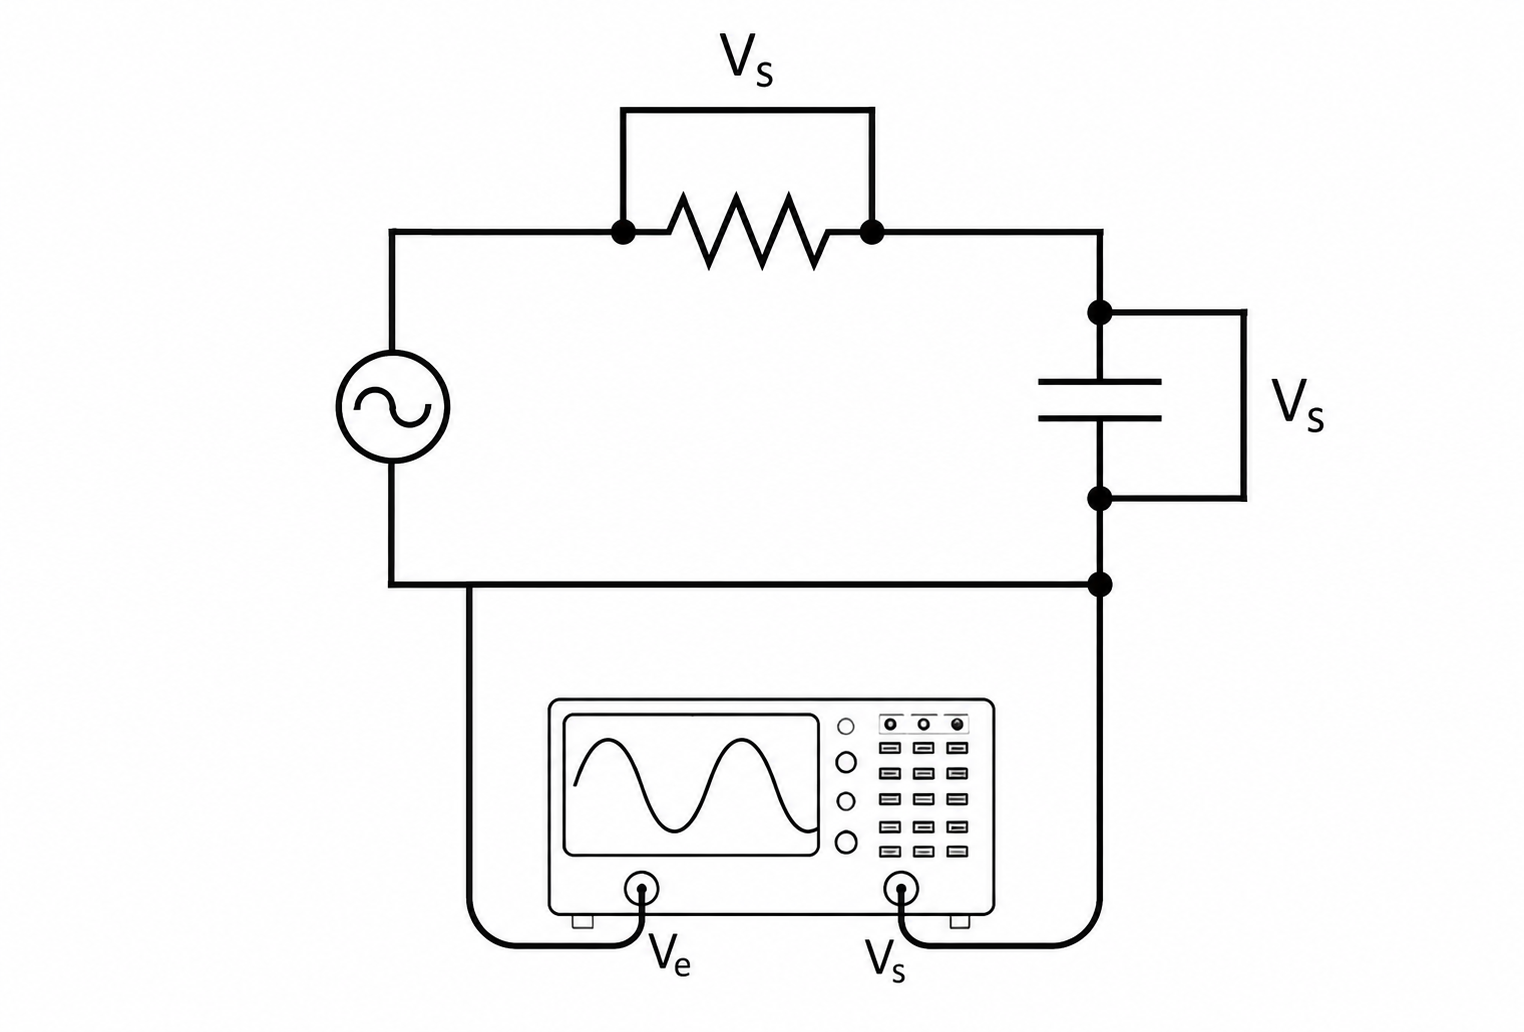
\includegraphics[width=\linewidth]{gráficos/circuitoRC.png}
        \caption{Circuito RC en serie.}
        \label{fig:circuitoRC}
    \end{subfigure}
    \hfill
    \begin{subfigure}[b]{0.40\linewidth}
        \centering
        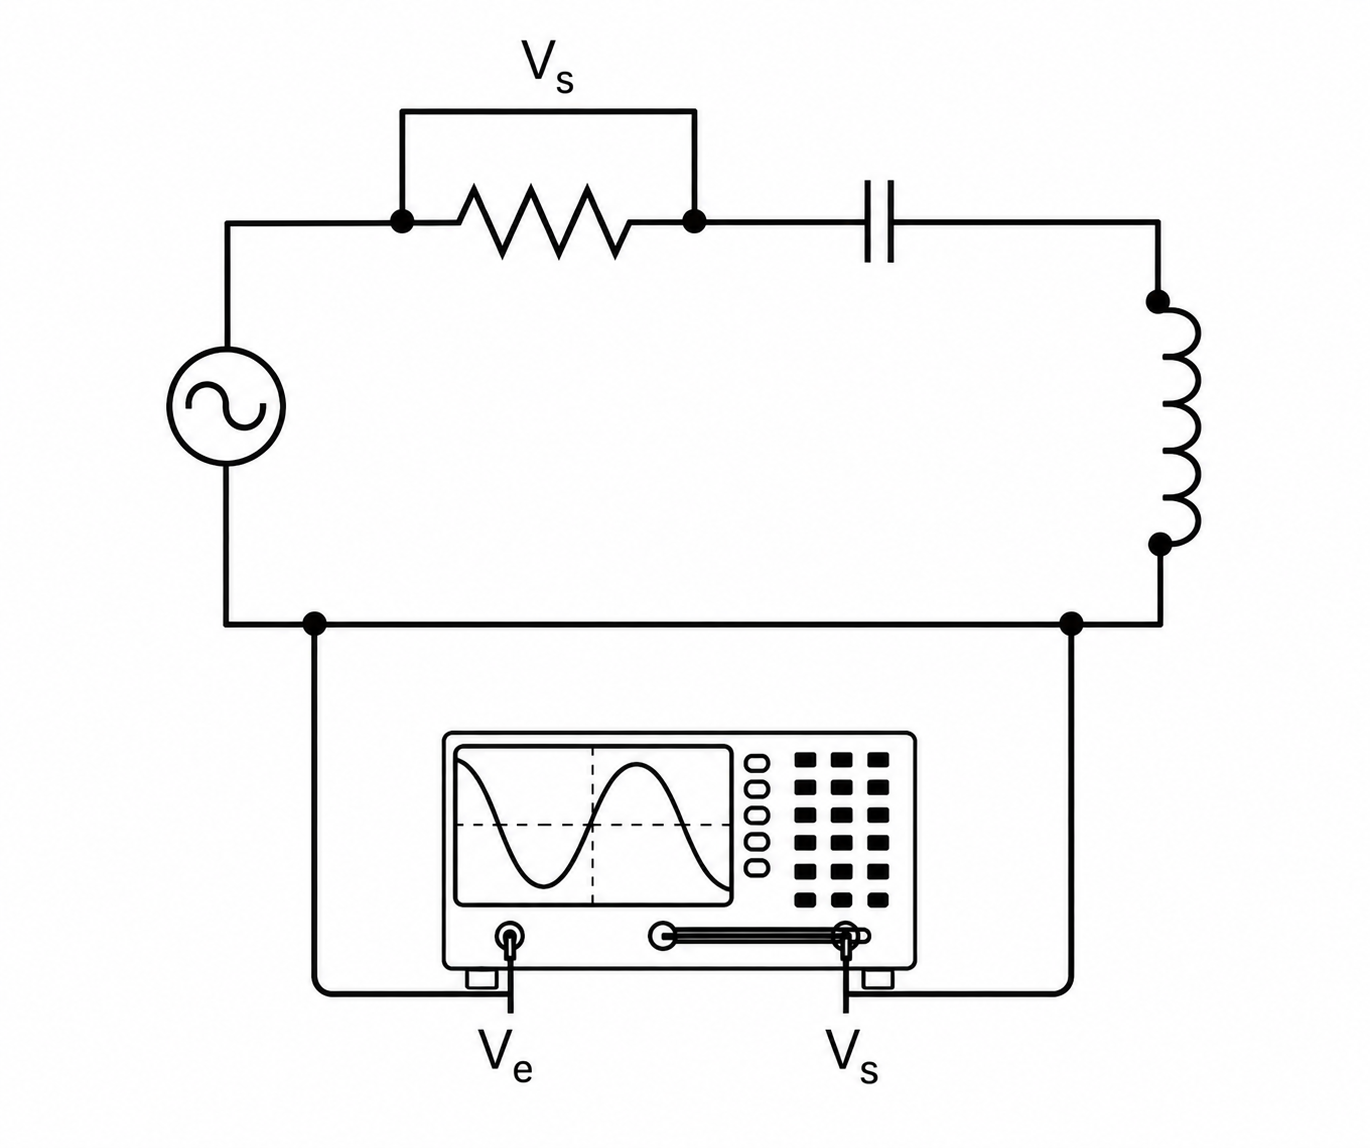
\includegraphics[width=\linewidth]{gráficos/circuitoRLC.png}
        \caption{Circuito RLC en serie.}
        \label{fig:circuitoRLC}
    \end{subfigure}
    \caption{Esquemas de los circuitos estudiados, en (a) circuito RC y en (b) circuito RLC. Se midió el voltaje de salida $V_s$ respecto del de entrada $V_e$, utilizando un osciloscopio, se señalan sus respectivas conexiones.}
    \label{fig:ambosCircuitos}
\end{figure}

Como señal de entrada se empleó una señal sinusoidal generada mediante un generador de funciones $Sinometer$ modelo VC2002 \cite{VC2002}, manteniendo amplitud constante y variando la frecuencia en el rango [0.1, 50] \SI{}{\kilo\hertz}. La señal de entrada $V_e$ y la señal de salida $V_s$, se registraron simultáneamente utilizando un osciloscopio $Tektronix$ modelo TDS 220 \cite{TDS200}. 

Para el circuito RC se realizaron dos configuraciones experimentales. En la primera, la señal de salida se midió sobre la resistencia, obteniendo la respuesta correspondiente a un filtro PA. En la segunda, la señal de salida se midió sobre el capacitor, obteniendo entonces la respuesta propia de un filtro PB. Con respecto al circuito RLC, la señal de salida se midió únicamente sobre la resistencia. En cada medición se registraron las amplitudes de las señales de entrada y salida, así como la diferencia temporal $\Delta t$ entre ambas. A partir de estos datos se calculó el desfasaje entre señales mediante la relación $\varphi=2\pi f \Delta t$, donde $f$ es la frecuencia de $V_e$ y $\omega=2\pi f$. Asimismo, se determinó el módulo de la función de transferencia como el cociente entre las amplitudes de salida y entrada a partir de la relación dada por \autoref{cociente}. 

Se construyeron diagramas de Bode, representaciones gráficas de la respuesta en frecuencia del sistema obtenidas mediante la representación del módulo de la función de transferencia en dB y la fase en grados, para ambas configuraciones del circuito RC. Esto se realizó debido a que la frecuencia de corte $\omega_0$ puede determinarse a partir de la intersección entre los comportamientos asintóticos de baja y alta frecuencia, tanto para la configuración PA como para la configuración PB, ya que la linealización de $\log\left| H(\omega) \right|$ resulta en dos rectas que se intersecan en dicha frecuencia. Bajo esta condición, para el PB  la recta correspondiente al régimen de bajas frecuencias se representa como una recta horizontal en 0 dB en el diagrama de Bode. Por otro lado, al
considerar el régimen de altas frecuencias se consigue una recta con pendiente negativa. Se realizó de manera análoga para el PA, siendo que el régimen de bajas frecuencias se aproxima mediante una recta de pendiente positiva y el de altas frecuencias con una recta a 0 dB . Además, se comparó este resultado con el valor esperado a partir de la condición $\left| H(\omega) \right|=\frac{1}{\sqrt{2}}$. 

En el caso del circuito RLC, se representó el módulo de la función de transferencia en función de la frecuencia angular, identificando la frecuencia de resonancia como aquella para la que $\left| H(\omega) \right|$  alcanza un máximo. La frecuencia de resonancia $\omega_r$ entonces, se obtuvo a partir del ajuste de los datos según la función dada por \autoref{eq:moduloRLC}. Se llevaron a cabo dos ajustes, uno fijando al parámetro $\tau$ al obtenido experimentalmente para el circuito RC, y otro dejando a $\tau$ libre, caracterizando un $\tau_{ef}$ efectivo del sistema. Un vez encontrada $\omega_r$, se determinó la inductancia del circuito mediante la relación $\omega_r=\frac{1}{\sqrt{LC}}$. 

Finalmente, para ambas configuraciones se construyeron diagramas de Nyquist, que representan gráficamente la respuesta del sistema según su geometría, a partir de  la parte imaginaria de $H(\omega)$ en función de su parte real. 

